\documentclass[12pt]{ociamthesis}  % default square logo 
%\documentclass[12pt,beltcrest]{ociamthesis} % use old belt crest logo
%|\documentclass[12pt,shieldcrest]{ociamthesis} % use older shield crest logo

%load any additional packages
\usepackage{amssymb}
\usepackage{amsmath}
\usepackage{url}
\usepackage[toc,page]{appendix}
\usepackage{graphicx}
\graphicspath{{./figures/}}
\DeclareGraphicsExtensions{.pdf,.png, .gif, .jpg}
\usepackage{qtree}
\usepackage{forest}
\usepackage{makecell}
\usepackage{xcolor}
\usepackage{colortbl}
\usepackage{fixltx2e}
\usepackage{array}
\newcolumntype{M}[1]{>{\arraybackslash}m{#1}}
\newcolumntype{N}{@{}m{0pt}@{}}

%============ BIBLIOGRAPHY AND REFS PACKAGES ========%
\usepackage{multibib}
\newcites{x}{References}
\newcites{sec}{Background Reading}

%============ for gloss overline ========%
\makeatletter
\newcommand{\OVER}[1]{$\overline{\hbox{#1}}\m@th$}
\makeatother

\newcommand{\TAG}{\textsuperscript}
\newcommand{\SUB}{\textsubscript}

% ========= for table stuff
\newcommand\Tstrut{\rule{0pt}{2.6ex}}       % "top" strut

% ============== stuff below is for header\footer
\usepackage{fancyhdr}
\pagestyle{fancy}
\fancyhead{}
\renewcommand{\sectionmark}[1]{\markright{\textit{#1}}}
\renewcommand{\chaptermark}[1]{\markboth{\arabic{chapter}.\ \textsc{#1}}{}}
\fancyhead[LO]{\leftmark}
\fancyhead[RE]{\rightmark}
%\fancyhead[R]{\rightmark}
%\fancyhead[L]{\leftmark}
\fancyhead[LE,RO]{\bfseries\thepage}
%\cfoot{\fancyplain{}{\thepage}}
\cfoot{}

% ============== FRONT PAGE =========== %
        
\title{Automated Visualised Translation from English to British Sign Language}

\author{Nicolaos Moscholios}             %your name
\college{Pembroke College}  %your college

\degree{Master of Computer Science}     %the degree
\supervisor{Dr. Joe Pitt-Francis}
\degreedate{Trinity 2016}         %the degree date

%end the preamble and start the document
\begin{document}

%this baselineskip gives sufficient line spacing for an examiner to easily
%markup the thesis with comments
\baselineskip=18pt plus1pt

\maketitle                  % create a title page from the preamble info

\begin{abstract}
A large number of people in the world today are born deaf and many rely on British Sign Language (BSL), the most widely used method of signed communication in the UK. BSL is structured in a completely different way to English and, like any language, it has its own grammar. In order to create a communication bridge between English speakers and individuals affected by deafness there have been attempts at building a formal model of translation. ...
\end{abstract}

\begin{acknowledgements}
I would like to thank...
\end{acknowledgements}

\begin{notes}
The work described in this thesis is available online at \url{nicmosc.com/bsltranslate}. Examples discussed throughout the report marked by an asterisk ($\ast$) can be viewed on the website. For demonstrative purposes it is highly suggested that the Examiner try those examples ..
\end{notes}

%\include{abstract}          % include the abstract
{\pagestyle{plain}
	\begin{romanpages}          % start roman page numbering
	%set the number of sectioning levels that get number and appear in the contents
	\setcounter{tocdepth}{5}
	\setcounter{secnumdepth}{5}
	\tableofcontents            % generate and include a table of contents
	\listoffigures              % generate and include a list of figures
	\listoftables
	\end{romanpages}            % end roman page numbering
\cleardoublepage}

%==================================================================================================================================================
%##################################################################################################################################################
%==================================================================================================================================================
%											   ##   
%											 ####   
%											   ##   
%											   ##   
%											   ##   
%											   ##   
%											 ###### 
%==================================================================================================================================================
%##################################################################################################################################################
%==================================================================================================================================================

\chapter{Introduction}
For most people around the world, communication is achieved orally by speaking. Unfortunately some are born deaf or are affected by hearing impairment with time. It is then necessary to use another medium of communication. Today there are about 1 million "functionally deaf" UK individuals \citex{website:bsl-stats}, that is, that require the use of sign language to converse. Additionally there are around 11 million people affected by some degree of hearing loss and while many benefit from hearing aids, sign language bypasses the need to speak, making it easy for everyone to understand each other.  

\section{Motivation}
The problem arises when hearing and Deaf individuals need to communicate. Deaf individuals are taught to read and write English from a young age, but it was found that they have difficulties understanding text with a reading level above that of primary school students \citex{paper:deaf-edu}. Thus it is not enough for hearing individuals to rely on written text to communicate with their community. More and more people are learning BSL even though they have perfectly fine hearing. There are certificates that can be obtained to work with Deaf individuals \citex{website:signature}. Taking lessons from BSL teachers and practising with the community helps to learn the language.

Online resources such as UCL's BSL Sign Bank \citex{website:bsl-sign-bank} and SignBSL.com \citex{website:sign-bsl} offer clips of signers showing words and phrases in BSL for learners and curious people?. The main issue is that they are highly static. Analogously to an English dictionary, it is only useful for looking up individual signs and not \textit{translating} phrases. Automated translation has been an ongoing challenge in the field of
computational linguistics, and we are finally seeing very positive results thanks to the recent developments in machine learning. Since spoken (written) languages are heavily dependent on their syntactic components, they are relatively easy to formalise in such a way that a machine can interpret a sentence and perform operations on it to transition from one language to another. More recently, there have also been attempts at doing so with signed languages such as ASL (American Sign Language) and BSL. Given that there is no formally typed grammar for BSL, it is not easy to find a model that encapsulates all key elements involved, such as facial expressions and eye gaze. In addition, since the language is only signed, the only way to see if an interpretation is correct, is through visual output. While some past implementations have been successful, due to the then high computational power necessary to run these systems, most of them are now outdated or have been left at a prototype stage. In 2006, IBM created a fully working system \citex{website:IBM} that allowed users to speak and see the translation from English to BSL in real time; however it has been disregarded and is not available any more. 

\section{Objectives}
This project will build upon previous work and attempt to solve the interlingual translation from English to British Sign Language by implementing a web application where signs are visualised through a virtual avatar. Behaviour will closely follow that of other established translation systems such as Google Translate where users can type a sentence and get a result in real-time. Through rule-based translation methods (discussed in section \ref{machine translation}) and 3D animation techniques the system will allow users to not only find out what a particular sentence corresponds to in BSL, but also learn and hopefully practice their skills. Figure \ref{fig:sys-overview} shows a conceptual overview of the system pipeline; this figure will be references multiple times throughout the report.

\begin{figure}[h]
	\centering
    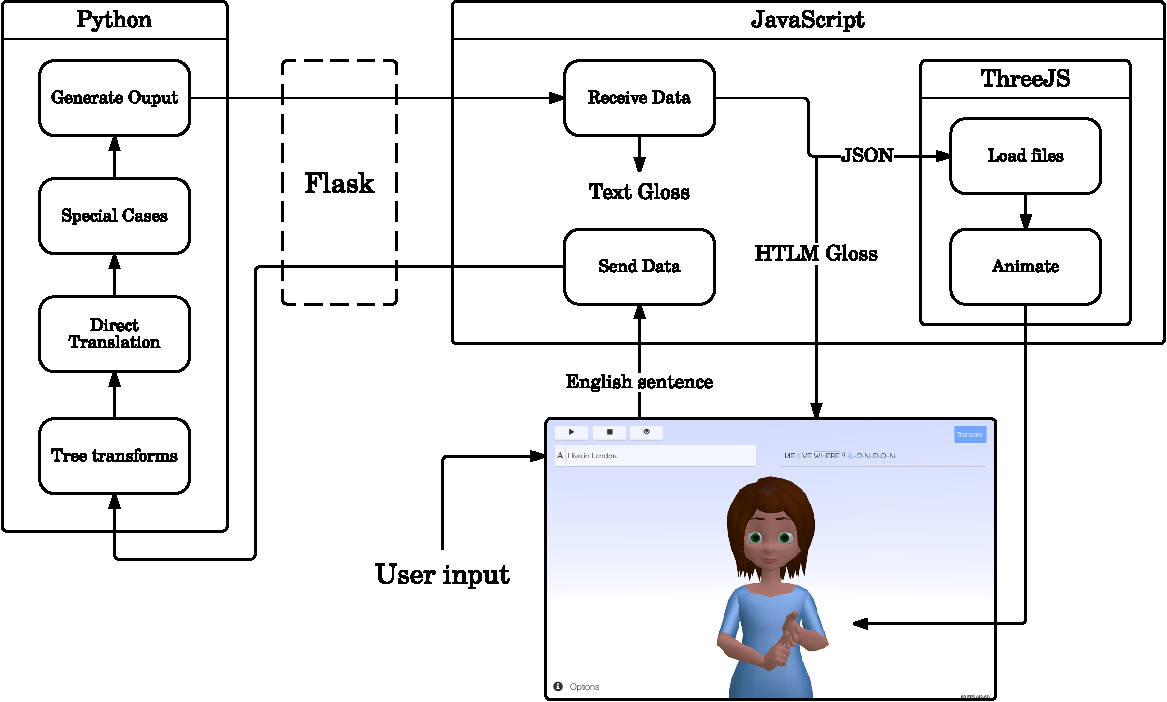
\includegraphics[scale=0.75]{chapter1/system-overview}
    \caption{Conceptual overview of the system}
    \label{fig:sys-overview}
\end{figure}

\section{Structure}
The report will read as follows: in chapter 2 we will give a brief introduction to the linguistics British Sign Language and its differences from written English, as well as existing methods of translation from written to written and from written to signed languages. Chapter 3 will cover the design choices for the system, that is, the development environment with the programming languages, the conceptual structure of the pipeline and the end-user interaction. Following up in chapter 4 we explain in detail the implementation of both the translation methods and the animation techniques utilised, as well as the communication between the two modules. Finally chapter 5 will discuss the evaluation of the system both in terms of translation accuracy and feedback from the user survey, while chapter 6 concludes the report along with project achievements, personal remarks and future work.

%==================================================================================================================================================
%##################################################################################################################################################
%==================================================================================================================================================
%											 #######  
%											##     ## 
%											       ## 
%											 #######  
%											##        
%											##        
%											######### 
%==================================================================================================================================================
%##################################################################################################################################################
%==================================================================================================================================================

\chapter{Background}
This chapter is separated in two main sections: an overview of British Sign Language, and Machine Translation theory and its particular applications in BSL translation. 
\section{British Sign Language: Linguistics Overview}
This section will give a short introduction to the linguistics of British Sign Language, including common grammar rules, its morphology and how it differs from written English. Please note that only the most general information is described here in order to follow the concepts discussed in chapter \ref{implementation} and other parts of the report, which are based on this theory. However it is not necessary to read this section before the one following as any approach that requires knowledge of BSL linguistics will reference this section for further understanding if necessary. The following examples and explanations are based on the book by Woll and Sutton, \textit{The Linguistics of British Sign Language: an Introduction}. \\

British Sign Language, often shortened to BSL, has been an officially recognised language since 2003 \citex{website:signature}. Like English, it has its own grammar \citex{website:deafness} and its own lexicon. While not as large as its written counterpart, there are enough signs to convey the same ideas in sign language, as many can be combined to create new meanings (\textit{compounds}, see section \ref{morphology}). However BSL is not the only signed language; each country has their own with different dialects by region. ...  

Since BSL can only be transmitted through signing, there is no formal written form. Many different formats exist such as Stokoe, designed for ASL by William Stokoe only for representing hand movements \citex{paper:stokoe} thus carrying no information about non-manual features, later adapted to BSL by Kyle and Woll \citex{book:bsl-stokoe}, HamNoSys (Hamburg Notation System) that can represent any signed language \citex{paper:hamnosys}, SignWriting which uses visual icons to represent parts of the body \citex{thesis:signwrite} and more. However the most commonly used method to represent sign language without needing to learn the notation (all of the above require additional knowledge to be decoded) is through \textit{gloss}. Gloss uses the most basic representation of the sign in its English written form. For example if one wants to describe a situation where a girl is eating an apple, the gloss would be GIRL EAT APPLE. The advantage of this notation is that we can clearly understand what a sentence means as we associate the sign to its English meaning. The main disadvantage though is that there is no information about the sign whatsoever, we only know that the particular sign for GIRL is signed first, followed by the sign for APPLE and so on. Table \ref{table:comparison} shows an example sign for every notation type.

Gloss notation also carries some information about non-manual features (see section \ref{non-man}) for example the sentence ``Where do you live?'' would be YOU LIVE \OVER{WHERE }\TAG{br}, where br represents a brow raise for asking questions. ?This is the format we will use for the rest of the report and it is what is used in the application as well?.

\begin{table}[ht]
\begin{center}
\begin{tabular}{| c | c | c | c | c | c |}
	\hline
	English & Sign & SignWrite & Stokoe & HamNoSys & Gloss \\ \hline
	\Large What? & \raisebox{-.5\height}{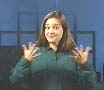
\includegraphics[scale=0.8]{chapter2/woman}}
    & \raisebox{-.5\height}{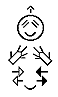
\includegraphics[scale=0.7]{chapter2/signwrite}}
    & \raisebox{-.5\height}{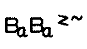
\includegraphics[scale=0.6]{chapter2/stokoe}}
    & \raisebox{-.5\height}{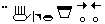
\includegraphics[scale=0.8]{chapter2/ham}}
    & \OVER{WHAT }\TAG{br}
    \\ \hline
\end{tabular}
\caption{Examples of different BSL written forms}
\label{table:comparison}
\end{center}
\end{table}

Let us now discuss the particular features of BSL and how it is structured as a language.

\subsection{Structure of sentences}
\label{structure}
In English, sentences follow very similar patterns. Most often we find a noun phrase followed by a verb phrase, each one containing information about the subject and the object (Fig. \ref{fig:english-sent}). BSL, just like English, has its own rules for ordering signs within a sentence. However many learners and signers speaking with learners of BSL sometimes employ the spoken English ordering to facilitate understanding. A sentence is divided in two basic parts: \textbf{subject}, the theme or topic, most often a noun, a noun phrase or a pronoun, and \textbf{predicate}, the rest of the sentence normally describing the action of the subject. BSL borrows some elements from English, such as the concept of pronouns, adjectives, verbs etc. but also includes \textit{proforms} and \textit{classifier predicates} which do not exist in English. 
\begin{figure}[h]
\Tree [.S
 	   	 [.NP 
			[.\textcolor{blue}{DT} The ] 
			[.\textcolor{blue}{JJ} large ] 
			[.\textcolor{blue}{NN} cat ] 
 	   	 ]
 	   	 [.VP 
 	   	 	[.\textcolor{blue}{VBP} sat ] 
			[.PP 
				[.\textcolor{blue}{IN} on ]
				[.NP 
					[.\textcolor{blue}{DT} the ] 	
					[.\textcolor{blue}{NN} mat ] 			
				]		
			] 	   	 
 	   	 ]
 	 ]
\caption{English sentence syntax tree}
\label{fig:english-sent}
\end{figure}
Proforms are ``anything that refers to, and stands in the place of, something previously identified'', that is, one may sign a word such as CAR first, and then when describing an action of the car such as ``driving in a zig-zag motion'' the dominant hand assumes the proform \textit{shape} associated with the car. Examples of hand shapes include `B' for vehicles and round/flat objects like PLATE (generally objects having 2 dimensions), `V' and `$\ddot{\text{V}}$' or `G' (one dimension) for MAN etc. Figure \ref{table:handshapes} shows examples for each\footnote{There are 22 handshapes in total and interestingly most of the shapes correspond to the ASL signed alphabet.}. When we use a specific handshape to describe the action or features of a word belonging in a specific group is what is called a classifier predicate. In another example we may want to sign ``The car goes under the bridge'', thus we would sign CAR and BRIDGE and then use the \textit{classifier} for car Veh-CL (vehicle classifier, represented by the B hand with palm facing down) and the bridge classifier 3D-CL ($\ddot{\text{B}}$ hand) to show the car moving under the bridge object.

\begin{table}[ht]
\begin{center}
\begin{tabular}{| c | c | c | c | c |}
	\hline
	B & $\ddot{\text{B}}$ & V & $\ddot{\text{V}}$ & G \Tstrut \\
	\raisebox{-.5\height}{
\includegraphics[scale=1]{chapter2/B}}
	& \raisebox{-.5\height}{
\includegraphics[scale=1.1]{chapter2/B2}}
    & \raisebox{-.5\height}{
\includegraphics[scale=1]{chapter2/V}}
    & \raisebox{-.5\height}{
\includegraphics[scale=1.1]{chapter2/V2}}
    & \raisebox{-.5\height}{
\includegraphics[scale=1]{chapter2/G}}
    \\ \hline
\end{tabular}
\caption{Some BSL proform handshapes}
\label{table:handshapes}
\end{center}
\end{table}
\textbf{Pronouns} are used similarly to written English but there are some differences. Firstly, there is no distinction between masculine or feminine. Instead a G shape hand is used, normally glossed as Index followed by a number to specify which part of space we are referring to. For example
\begin{flalign*}
&\text{John told Mary that he loved her} \\
&= \text{-J-O-H-N- Index\SUB{1} TELL -M-A-R-Y- Index\SUB{2} Index\SUB{1} LOVE Index\SUB{2}}\tag{$\ast$}
\end{flalign*}
Subject Verb Object (SVO) is the preferred word order in spoken English, while SOV is more common in BSL. Yet, as mentioned previously many learners prefer to use SVO when signing. This works most of the time however some verbs require an SOV construct such as ME PIZZA EAT as the verb EAT is modified by the type of object that is being eaten. In other words the sign for eating a pizza will differ from the one when eating pasta.

\subsection{Morphology and Morphemes}
\label{morphology}
A morpheme in BSL is considered as the smallest unit of meaning in a word or sign. We can combine them to form signs that have several meaningful parts but are still considered a single sign. Figure \ref{fig:morphemes} shows the BSL sign morphology tree. We distinguish between \textit{monomorphemic} signs (cannot be further subdivided) like TRUE, SAY, MOUSE and \textit{polymorphemic} which are a combination of 2 or more morphemes. For example PROMISE is the combination of the sign for SAY and TRUE, or CHECK = SEE + MAYBE. We also categorise morphemes as \textbf{Free} that can stand alone (i.e. monomorphemes like RED, TRUE, SAY) and \textbf{Bound} which have a meaning but \textit{must} be combined with at least one other morpheme, and \textbf{Plural} morphemes.  

\begin{figure}[h]
\begin{forest}
[Signs
	[\makecell{Monomorphemic \\ (free morphemes)}]
    [Polymorphemic 
		[\makecell{2 (or more) free \\ morphemes "compounds"}] 
		[\makecell{Combination of bound \\ and free morphemes}] 
		[\makecell{Combination of 2 \\ (or more) bound morphemes}]
	]
]
\end{forest}
\caption{BSL sign morphology schema}
\label{fig:morphemes}
\end{figure}

Free morphemes are often combined to form a \textbf{compound}, a sign with a different but related meaning. Some are borrowed from English like BALANCE-SHEET while others aren't: BLOOD = RED + FLOW, TIGER = ZEBRA + ANIMAL. When combining free morphemes, the compound must appear as similar as possible to a single sign, thus the originals are modified by rapid transitioning (both signs are accelerated), the initial hold of the first sign and any repeated movement in the second sign are lost. For example if MOTHER = -M-M- and FATHER = -F-F- then PARENTS = -M-F- and not -M-M-F-F-.

Bound morphemes must be attached to another free morpheme. The sign for DRIVE-CASUALLY combines the free morpheme DRIVE (verb) and bound CASUALLY, since we need to specify what action is being performed in a casual manner. Similarly the agreement verb ASK (see section \ref{verbs}) requires the subject and object such as YOU and ME (both free morphemes) to form the complete verb YOU-ASK-ME.

Plural morphemes include both free and bound morphemes and can carry information about nouns and verbs. In English this trait corresponds to the terminal \textit{-s}. In ``cats'' we find cat + s where [s] is the form of a \textit{bound} morpheme: it cannot stand alone. However in BSL we cannot just add a terminal to the sign. Instead plural morphemes can be attached to a sign, modify the sign itself or appear separately. For example the plural ``children'' can be signed as CHILD repeated multiple times, or we can  sign TWO CHILD if we know there are 2 of them, or otherwise using pronouns like CHILD THEM to mean that there are more than one.

Adjectives also carry some morphological information as they convey a particular feature of nouns or pronouns. Adjectives can be \textbf{attributive} when they occur in the noun phrase and appear before, after or within a noun e.g. SHIRT WHITE, or \textbf{predicative} when they act like a verb e.g. MAN Index\textsubscript{3} TALL where the man is ``executing'' the action of being tall. However they are not used very often, since signs can be modified directly instead; the sign for BOX involves making a square shape with both hands, however SMALL-BOX and LARGE-BOX will modify the movement for the base sign by leaving less or more space between the hands respectively. Signs that cannot be directly modified make use of the normal adjective signs (there is indeed a sign for both small and large) and can be preceded by a premodifier like VERY, QUITE etc. Adjective signs in comparative (\textit{-er}) and superlative (\textit{-est}) form are modified by making the initial hold very long and tense, followed by a rapid release, where the degree of tension depends on the modifier.

\subsection{Verbs}
\subsubsection{Tense, Aspect and Mood}
In English when we want to refer to an action that will happen in another point in time we conjugate the verb (``He will go home'') or use words that convey the same idea (``He's going home tomorrow''). BSL uses WILL and TOMORROW as keywords to show an action happening at a different time. Furthermore, time is always set at the beginning of a sentence and is also emphasized through eye gaze (see section \ref{eye-gaze}). E.g. 
\begin{flalign*}
&\text{I went to London yesterday} = \text{YESTERDAY ME GO -L-O-N-D-O-N-} \tag{$\ast$}
\end{flalign*}
Aspect is the internal timing of things and describes if something is happening relative to another event, how long it went on for, if it is not finished yet and so on. For example if we're describing the action of someone looking for a long time, the sign LOOK-FOR-A-LONG-TIME is simply the base sign LOOK with the hands kept in position for longer and a facial expression with eyes open wider.

What in English is used as modal auxiliaries like \textit{may, can, shall, must} is performed by signing the corresponding signs either before or after the verb e.g. CAN HAVE, modifying the verb itself by making it stronger and bigger depending on the mood e.g. MUST-ASK is stronger than CAN-ASK, or by using facial expressions.
\subsubsection{Verb types}
\label{verbs}
In BSL we define two types of signing space: topographic and syntactic. The former describes a real world location according to the \textit{actual} features. For example if standing outside one may directly point at a tree they want to describe. On the other hand, the latter is a space ``created within the language'' and may not reflect the real world since it is used figuratively. In the sentence
\begin{flalign*}
&\text{I gave my aunt a book} = \text{AUNT Index\SUB{3} Index\SUB{1} BOOK\SUB{1} GIVE-BOOK\SUB{3}}
\end{flalign*}
The real aunt is not where the signer is pointing (Index\SUB{3}). Furthermore, we distinguish between 3 types of verbs:
\begin{itemize}
	\item Plain verbs: these signs show little modification and do not move through space. Any information about what and how many entities the verb describes is given through pronouns. E.g. ``I like him'' is signed ME LIKE HIM i.e. all signs are separated.
	\item Agreement verbs: can be modified to show additional information and are signed in syntactic space. ``I give you ...'' is ME-GIVE-YOU, where the hand moves \textit{from} the ME position \textit{to} YOU with the specific handshape (verb stem) for GIVE; pronouns are not signed individually. This movement has 3 steps: subject agreement marker, verb stem and object agreement marker. This means that in YOU-GIVE-ME the movement is essentially reversed.
	\item Spatial verbs: use topographic space instead and are used to describe a trajectory, speed of movement and location of an action. Examples include RUN-DOWNSTAIRS, DRIVE-TO etc. Most often these use classifier predicates to describe surrounding entities (see section \ref{structure}).
\end{itemize}

\subsection{Questions and Negations}
\label{qneg}
When asking a question, the whole sentence is accompanied by a brow raise, a head tilt and opened eyes. The question ``Do you like tea?'' is \OVER{YOU LIKE TEA }\TAG{q}. Some questions only include a brow raise on parts of the sentence, such as in ``You have three children right?'' = THREE CHILD HAVE \OVER{RIGHT }\TAG{q} since we are asking for confirmation.

Wh- question, which include \textit{what, why, where, when, who, which, how} usually follow the same rule as the above where only the wh- word is accompanied by a question facial expression. For example:
\begin{flalign*}
&\text{Who are your parents?} = \text{YOUR -M-F- \OVER{WHO }\TAG{q}} \tag{$\ast$} \\
&\text{Where did he go?} = \text{Index\SUB{1} GO \OVER{WHERE }\TAG{q}} \tag{$\ast$}
\end{flalign*}
However questions can also be used in sentences which are not questions by nature. In fact the following
\begin{flalign*}\tag{$\ast$}
&\text{I love John because he's nice} = \text{ME LOVE -J-O-H-N- \OVER{WHY }\TAG{q} Index\SUB{1} NICE} \\
&\text{I won't go to the beach if it'll rain tomorrow} \\
&= \text{\OVER{TOMORROW RAIN}\TAG{q} ME \OVER{NOT GO }\TAG{neg} BEACH} \tag{$\ast$}
\end{flalign*}
essentially turning the sentence into a rhethorical question. The same happens when we try to describe the state of an object or person like
\begin{flalign*}
&\text{The keys are in the kitchen} = \text{KEYS \OVER{WHERE }\TAG{q} KITCHEN} \\
&\text{I live in Oxford} = \text{ME LIVE \OVER{WHERE }\TAG{q} -O-X-F-O-R-D} \tag{$\ast$}
\end{flalign*}

Sentences that contain negations are signed considering three main elements: \\
\textbf{Facial expression}: the lips are pushed out and the eyes are narrowed \\
\textbf{Head movements}: the head turns to the side and is held there (accompanies a specific sign) or alternates between the left and right sides. The latter can negate both whole sentences or single signs e.g.
\begin{flalign*}
\text{I'm not eating pizza} = & \text{\OVER{ME PIZZA EAT }\TAG{neg}} \\
&\text{ME PIZZA \OVER{EAT }\TAG{neg}} \\
&\text{ME PIZZA EAT \TAG{neg} }
\end{flalign*}
\textbf{Negation signs}: these are specific hand gestures to show that a negation is happening, the most common ones are a flat hand, palm down twisting up following a verb or adjective (often used as a suffix with SEE+neg, HAVE+neg for denial of possession or experience) and the NOT sign. Thus the previous example can also be written as
\begin{flalign*}
\text{I'm not eating pizza} = & \text{ME PIZZA \OVER{NOT EAT}\TAG{neg}}
\end{flalign*}
Additionally, some signs when negated are completely different from the original and are not just preceded by NOT and the \textit{neg} expression. For example the verb ``know'' is performed by the dominant hand's fist with the thumb up tapping on the forehead, while its negation NOT-KNOW sees the two flat hands moving away from the forehead.

\subsection{Fingerspelling}
Fingerspelling is the action of using the signed alphabet to spell out a word, normally borrowed from English. The most general rule for figerspelling is that if the word is less than 3-4 letters long it is spelled in full, otherwise it can be abbreviated. The fingerspelling notation in gloss form is -B-B-C or -b-b-c- (example for the commonly known broadcasting company). There exist a few abbreviation rules however the most common ones are:
\begin{itemize}
	\item Using the first syllable e.g. January = -J-A-N-
	\item When the second letter is `h' we retain the first 2 e.g. chapter = -C-H-
	\item We can also use the first and last letter (mainly used for places) e.g. Glasgow = -G-W-
\end{itemize}
However if an unknown word is introduced in a context for the first time, such as personal name or a place name, then it is first spelled in full, and the following time the abbreviation is used. The name Hannah may be signed as -H-A-N-N-A-H- first and then just as -H-. On the other hand it is not uncommon for signers to use body/character features to refer to someone. For example if I would like to talk about a person that wears glasses, I would first need to sign their full name, followed by the sign for glasses. After setting that context the listener would know that every time GLASSES is signed, that person is being referred to.

\subsection{Non-manual features}
\label{non-man}
Non-manual features represent any action performed by the signer which is not performed by the hands and are used to represent spoken language mouth patterns in combination with signs, enacting actions and setting the context like verb tenses and questions. These are very important in BSL and are often mistakenly neglected by (in common knowledge/culture??)
\subsubsection{Spoken and Oral Components}
\label{so-components}
Spoken components are used to better identify the sign being used. Nouns that are fingerspelled are also mouthed when the last letter is signed; this also applies to abbreviated signs i.e. only one letter is signed but the whole word is mouthed. They are also extremely useful with homonyms, since only through mouthing it is possible to distinguish two meanings of a sign that has the same gestures e.g. FINLAND and METAL. The mouthing shape is borrowed from the English spoken version of the words.

Oral components enact real-life actions such as laughing or biting, where the sign is entirely mouthed (the hands are not involved, although there are manual versions of such actions as well). Additionally, mouthing can be used to represent negations as described in section \ref{qneg}.
\subsubsection{Facial Expressions and Head Movements}
Facial expressions are used to mark a question or a negation (as seen above) and to show emotions e.g.
\begin{flalign*}
\text{I was happy when dad arrived} = & \text{\OVER{ME HAPPY }\TAG{happy} WHEN -D-D- ARRIVE}
\end{flalign*}
They are also used in combination with a head nod to mark the topic. The topic can be \textit{temporal} when describing a situation in time such as ``When I$\ldots$'', \textit{spatial} and \textit{nominal} when describing a location or an entity. Most often said entity is the subject of the sentence thus
\begin{flalign*}
\text{The dog chased the cat} = & \text{\OVER{DOG }\TAG{hn} CAT CHASE}
\end{flalign*}
where hn stands for head nod.

\subsubsection{Eye Gaze}
\label{eye-gaze}
Eye gaze plays an important role during signing because of multiple reasons:
\begin{itemize}
	\item Lexical distinction: some signs such as GOD and BOSS are signed in the same way (homonyms) and are distinguished by the eye gaze; when signing GOD the eyes look upwards, similarly to how spoken components are used (see section \ref{so-components}.
	\item In conjunction with location and movement: the sign for HE/SHE (glossed as Index) may be in the same location as the sign for YOU but the eyes pointing somewhere else than the listener imply we are discussing another person. In addition the eyes follow the hand during movements e.g. when describing a rolling ball. 
	\item To mark time: in conjunction with a movement of the head, looking on the side can indicate the past, ahead or down indicates present, while looking up indicates the future.
\end{itemize}

\section{Machine Translation}
\label{machine translation}
Now that the necessary background in BSL linguistics has been laid out, let us discuss machine translation and how it is applied to signed languages. \\

Translation between written languages has been an ongoing research topic in the field of computational linguistics. The basic idea is that we wish to find relations between the syntactic components of the source and target language, and then model them in a way that a machine can understand it. There exist currently two main automated translation approaches: statistical and classical. Statistical MT is more recent than the latter, and has become very popular in recent years thanks to the advancements in machine learning. It is based on the concept of analysing huge bilingual corpora, which are essentially lists of sentences in the source language, with each having a set of possible reference translations. Classifiers are trained on these corpora and assign a probability of translation for each word in the sentence: this technique is called \textit{word alignment} (Fig. \ref{table:alignment}). Each word from the source sentence is assigned 0 or more words from the target. 

\begin{table}[ht]
\begin{center}
\begin{small}
\begin{tabular}{l|M{0.5cm}|M{0.5cm}|M{0.5cm}|M{0.5cm}|M{0.5cm}|M{0.5cm}|M{0.5cm}|M{0.5cm}|M{0.5cm}|N}
		\multicolumn{1}{l}{}& \multicolumn{9}{l}{Maria no \hphantom{a} dio \space una bofetada a \space la \space bruja verde}\\ 
        \cline{2-10}
        Mary & \cellcolor{black} & & & & & & & & \\ [12pt]
        \cline{2-10}
        did & & \cellcolor{black} & & & & & & & \\ [12pt]
        \cline{2-10}
        not & & \cellcolor{black} & & & & & & & \\ [12pt]
        \cline{2-10}
        slap & & & \cellcolor{black} & \cellcolor{black} & \cellcolor{black} & & & & \\ [12pt]
        \cline{2-10}
        the & & & & & & & \cellcolor{black} & & \\ [12pt]
        \cline{2-10}
        green & & & & & & & & & \cellcolor{black} \\ [12pt]
        \cline{2-10}
        witch & & & & & & & & \cellcolor{black} & \\ [12pt]
        \cline{2-10}
    \end{tabular}  
\end{small}
\caption{Word alignment English-Spanish}
\label{table:alignment}
\end{center}
\end{table}

However statistical MT is only possible when large amounts of parallel data are available. In the case they are not, other methods are required. Classical (or Rule-Based) machine translation requires deep understanding of both the source and target language in order to work. It involves the creation of ``rules'' that closely follow the syntactic and semantic constructs of both languages. The Vaquois triangle illustrates the multiple techniques, often combined, in rule-based translation (Fig. \ref{fig:vaquois}). 

\textbf{Direct translation} stands at the lowest level and is simply an equivalence relation between the words in the source and target languages. This step is usually performed via a dictionary lookup: word to word translation corpora are much more common than whole sentences. \textbf{Transfer} is a process that involves the \textit{transformation} of the target language structure into a another that more similarly resembles the target. Syntax trees can be generated by analysing both languages and then transforming the source to the specification of the target. From there direct translation can be applied to achieve a complete translation. Finally \textbf{interlingua}, while similar to transfer, is the transformation of the source into a universal representation that can be applied to any language. This is most useful when translation needs to occur both from and to the source and target.

\begin{figure}[h]
	\centering
    \includegraphics[scale=1]{chapter2/vaquois}
    \caption{Vaquois triangle for Rule-Based MT}
    \label{fig:vaquois}
\end{figure}
While statistical MT approaches usually achieve much higher accuracy than non-statistical methods because of the sheer amount of data used in the process, there have been multiple successful attempts at creating rule-based systems to cover languages with little or no corpora, even though they do prove to be much more time consuming to build and maintain \citex{paper:auto-refinement}. The most popular open-source system currently using shallow-transfer rules is Apertium\footnote{https://www.apertium.org}. It uses a language-independent specification so that resource-poor language pairs such as Serbo-Croatian/Macedonian can be added with time \citex{paper:serbo-macedonian}. A more recent approach has been that of \textit{hybrid} MT, where both statistical and rule-based methods are combined to achieve more flexibility and accuracy, sometimes using rules to correct the output of the statistical module \citex{paper:hybrid} \citex{paper:open-source} or by using medium sized corpora to induce rules to later be used with unseen sentences\citex{paper:inducing-translation} \citex{paper:inferring-transfer} \citex{paper:whats-in-rule}.

\subsection{MT with Signed Languages}
\label{existing methods}
Sign languages (including BSL and ASL) are visual-spatial by nature, hence there exists no real textual corpora. For this reason, many of the existing approaches have been rule-based rather than statistical, with some exceptions. Here we discuss the most successful approaches at translating sign languages, their advantages and drawbacks. 

\textbf{ZARDOZ} is a cross-modal translation system based on artificial intelligence using a blackboard control structure, where a common knowledge base is updated by workers as more solutions are found \citex{paper:zardoz}. The solution ultimately being an interlingual representation of the source translation (Fig. \ref{fig:zardoz}). Its main advantage is the ability to translate from English into any SL, such as Japanese, American and Irish Sign Language\citex{paper:zardoz-challenges}. To animate the output they use a virtual signing doll and calculate signing space to place the hands. However it is missing a sign lexicon i.e. a dictionary of signs, and there is no evaluation of the system in terms of accuracy or quality of the signing.
\begin{figure}[h]
	\centering
    \includegraphics[scale=1]{chapter2/interlingua}
    \caption{Interlingua representation using ZARDOZ}
    \label{fig:zardoz}
\end{figure}

\textbf{ViSiCAST} is a transfer based system from English to BSL that uses the HamNoSys phonetic transcription notation \citex{paper:drt}\citex{paper:prototype-text}. It involves 1) syntactic parsing using the Carnegie Mellon University link grammar parser, 2) semantic transfer i.e. the conversion to the SL structure from written English (here the data resembles an interlingua), and 3) the generation of SiGML\footnote{Signing Gesture Markup Language, an XML compliant representation of HamNoSys}. The output is then used to generate the video animation. Each sign stored as SiGML was animated using gesture tracking software for both the face and body movement, making the resulting signing very realistic. While there are no available accuracy results, the system has been tested in face-to-face scenarios in UK post offices with successful outcomes.

\textbf{TEAM}, another rule-based method dating 2000, is one of the first systems to use an augmented gloss representation of signs to generate its output. Through synchronous tree-adjoining grammars they convert the syntax trees of the source to the target language representation. In addition, embedded parameters help model the non-manual features such as facial expressions as well as Effort and Shape, which include speed, weight and spatial information of signs \citex{paper:team}. 

One of the few purely statistical systems is described in \citex{paper:statistical-sl}. Using only word alignment techniques, the authors state that their system is the most accurate translation system from English to ASL. Figure \ref{table:sl-alignment} shows how word alignment works with SL gloss. The main downside to this approach is that through word alignment there is no transfer of non-manual information, especially since their representation uses basic gloss. In addition the corpus the system was tested on is restricted and thus does not allow for great flexibility. \textbf{MaTrEx} \citex{paper:manual-labour} is another data-driven system, used in the development of software to be used in airports \citex{paper:joining-hands}.

\begin{table}[ht]
\begin{center}
\begin{small}
\begin{tabular}{l|M{0.5cm}|M{0.5cm}|M{0.5cm}|M{0.5cm}|N}
		\multicolumn{1}{l}{}&\multicolumn{4}{l}{\footnotesize YOU CAKE EAT ?}\\ 
        \cline{2-5}
        Did & \cellcolor{black} & & & \\ [12pt]
        \cline{2-5}
        you & \cellcolor{black} & & & \\ [12pt]
        \cline{2-5}
        eat & & & \cellcolor{black} & \\ [12pt]
        \cline{2-5}
        the & & \cellcolor{black} & & \\ [12pt]
        \cline{2-5}
        cake & & \cellcolor{black} & & \\ [12pt]
        \cline{2-5}
        ? & & & & \cellcolor{black} \\ [12pt]
        \cline{2-5}
    \end{tabular}  
\end{small}
\caption{Word alignment English-ASL}
\label{table:sl-alignment}
\end{center}
\end{table}

Ultimately, while all of the above manage to achieve some sort of translation from English to signed languages, none have been developed with portability in mind. The software needs to be either installed on a computer or a server making it only available to a handful of stakeholders. One interesting project tackles this by creating a mobile application to translate on the go \citex{paper:mobile-SL}. Signs are stored in a database and when a request to translate is made, the analysis of the sentence, translation and construction of the video output is done remotely. In addition, a special animation software was made available for users to create their own signs and add them to the dictionary. However this means translation is only available through the app installed on a phone, and the small screen of hand held devices makes it difficult to properly see the animations. Furthermore, only video is returned to the user, meaning there is no freedom of view (such as changing to a first person perspective, like was done in \citex{paper:3d-virtual-agent}). To our knowledge, there is no cross-platform, online translation tool currently available  to translate from English to BSL. ... Our goal is to create a real-time translation tool available to anyone, anywhere

\section{Personal Work}
It is necessary to mention that I have already worked on Sign Language with Animation. For my undergraduate project I created a system to teach BSL virtually, although this one only displayed a set of precomputed animations (animations were simply rendered in real time) and did not include any linguistics nor did it interpolate between signs. The architecture used to build the animation components was not efficient and did not fully exploit the features offered by OpenGL (which I will partially use again, through JavaScript). Since I wanted to learn more about skeletal animation I built everything from scratch in Java, something I would not do now considering the online environment and time restrictions imposed by the other aspects of the project. While I have not reused any previous material, I have used the knowledge I learnt from it in order to avoid repeating mistakes.
\section{Summary}
In this quite extensive chapter we have presented the basic linguistics concepts of BSL to give an idea of the complex elements to be considered when building a translation system for signed languages. We have also discussed existing approaches to this problem using a range of techniques, their drawbacks and benefits. In the next chapters the knowledge laid out in this chapter will be used to construct an online, cross-platform tool to translate from English to BSL.

%==================================================================================================================================================
%##################################################################################################################################################
%==================================================================================================================================================
%											 #######  
%											##     ## 
%											       ## 
%											 #######  
%											       ## 
%											##     ## 
%											 #######  
%==================================================================================================================================================
%##################################################################################################################################################
%==================================================================================================================================================


\chapter{Design}

\section{Language Choice}
\section{Translation}
\section{User Interface}
	\subsection{User Interaction}
\section{Summary}

%==================================================================================================================================================
%##################################################################################################################################################
%==================================================================================================================================================
%											##        
%											##    ##  
%											##    ##  
%											##    ##  
%											######### 
%											      ##  
%											      ##   
%==================================================================================================================================================
%##################################################################################################################################################
%==================================================================================================================================================


\chapter{Implementation}
\label{implementation}

\section{Rule-Based MT in Python}
	\subsection{Pipeline}
	\subsection{System Components}
		\subsubsection{Grammar Tree Transforms}
		Here remember to show a diagram of Marshall and their pipeline with word net, parser etc.
		\subsubsection{Direct Translation}
		\subsubsection{Special Cases}
		\subsubsection{Output}
	
\section{Animation in ThreeJS}
	\subsection{Blender}
		\subsubsection{Model}
		\subsubsection{Skeletal Animation}
	\subsection{Data Format}
		\subsubsection{JSON Formatter}
	\subsection{Animation Engine}
		\subsubsection{Pipeline}
		\subsubsection{ThreeJS}
	
\section{Interlingual Communication with Flask}
	\subsection{Python to JavaScript}

\section{Summary}
			
%==================================================================================================================================================
%##################################################################################################################################################
%==================================================================================================================================================
%											######## 
%											##       
%											##       
%											#######  
%											      ## 
%											##    ## 
%											 ######  
%==================================================================================================================================================
%##################################################################################################################################################
%==================================================================================================================================================


\chapter{Evaluation}

\section{Translation}
 Given the above consideration of SiGML evalu- ation, it appears that until a more appropriate evaluation method is developed, glosses are the most effective means of translating SLs.29 However, we must bear in mind the caveat that all these means of representation may not appropriately encapsulate inflectional and other linguistic information that may be integral to the understand- ing of a signed utterance (FROM \citex{paper:manual-labour}).
	\subsection{BLEU}
	Give a table comparing this to other methods described in background
\section{Animation}
\section{Survey}
\section{Feedback}

%==================================================================================================================================================
%##################################################################################################################################################
%==================================================================================================================================================
%											 #######  
%											##     ## 
%											##        
%											########  
%											##     ## 
%											##     ## 
%											 ####### 
%==================================================================================================================================================
%##################################################################################################################################################
%==================================================================================================================================================


\chapter{Conclusion}

\section{Improvements}
	Here mention the possible motion capture projects to improve animations
	\subsection{Handling of Agreement Verbs}
	\subsection{Classifiers}
	Here mention Huenerfauth and his system in more detail to discuss classifiers \citex{thesis:generating-classifiers}\citex{paper:multi-path}
\section{Expansion}

%===================== APPENDIX ===================%

%now enable appendix numbering format and include any appendices
{\pagestyle{plain}
\appendix
\chapter{Extra code (appendix)}

%===================== REFREENCES ===================%
%next line adds the Bibliography to the contents page
\addcontentsline{toc}{chapter}{References}
\bibliographystylex{plainurl}
\bibliographyx{references.bib}
\newpage

\addcontentsline{toc}{chapter}{Background Reading}
\nocitesec{*}
\makeatletter
\renewcommand\@biblabel[1]{}
\makeatother
\bibliographystylesec{plainurl}
\bibliographysec{bibliography.bib}
\cleardoublepage}

\end{document}